\section{ERNIE 1.0} \label{sec:ERNIE_1}

\subsection{Motivation for ERNIE 1.0}

Co-occurrence count models like \nameref{sec:Word2Vec}, \nameref{sec:Glove}, and \nameref{sec:BERT} create word vector representations only via surrounding contexts, not also through prior knowledge in the sentence, and thus fail to capture relations between entities in a sentence. Consider the following training sentence: 

{\normalsize \textit{``Harry Potter is a series of fantasy novels written by J. K. Rowling."}}

Using co-occurring words ``J.", ``K.", and ``Rowling", BERT is limited to predicting the token ``K." but utterly fails at recognizing the whole entity \emph{J. K. Rowling}. A model could use mere co-occurrences to predict missing entity \emph{Harry Potter} but it would not be making use of the relationship between the novel and its writer. 

\textbf{ERNIE 1.0} comes to the rescue here. \textbf{ERNIE (Enhanced Representation through Knowledge Integration)} extrapolates the relationship between the \emph{Harry Potter} entity and \emph{J. K. Rowling} entity using implicit knowledge of words and entities, and then uses this relationship to predict that \emph{Harry Potter} is a series written by \emph{J. K. Rowling} (Sun et al., 2019a). 



%\begin{figure}[h]
%\vspace{-5pt}
%\centering
%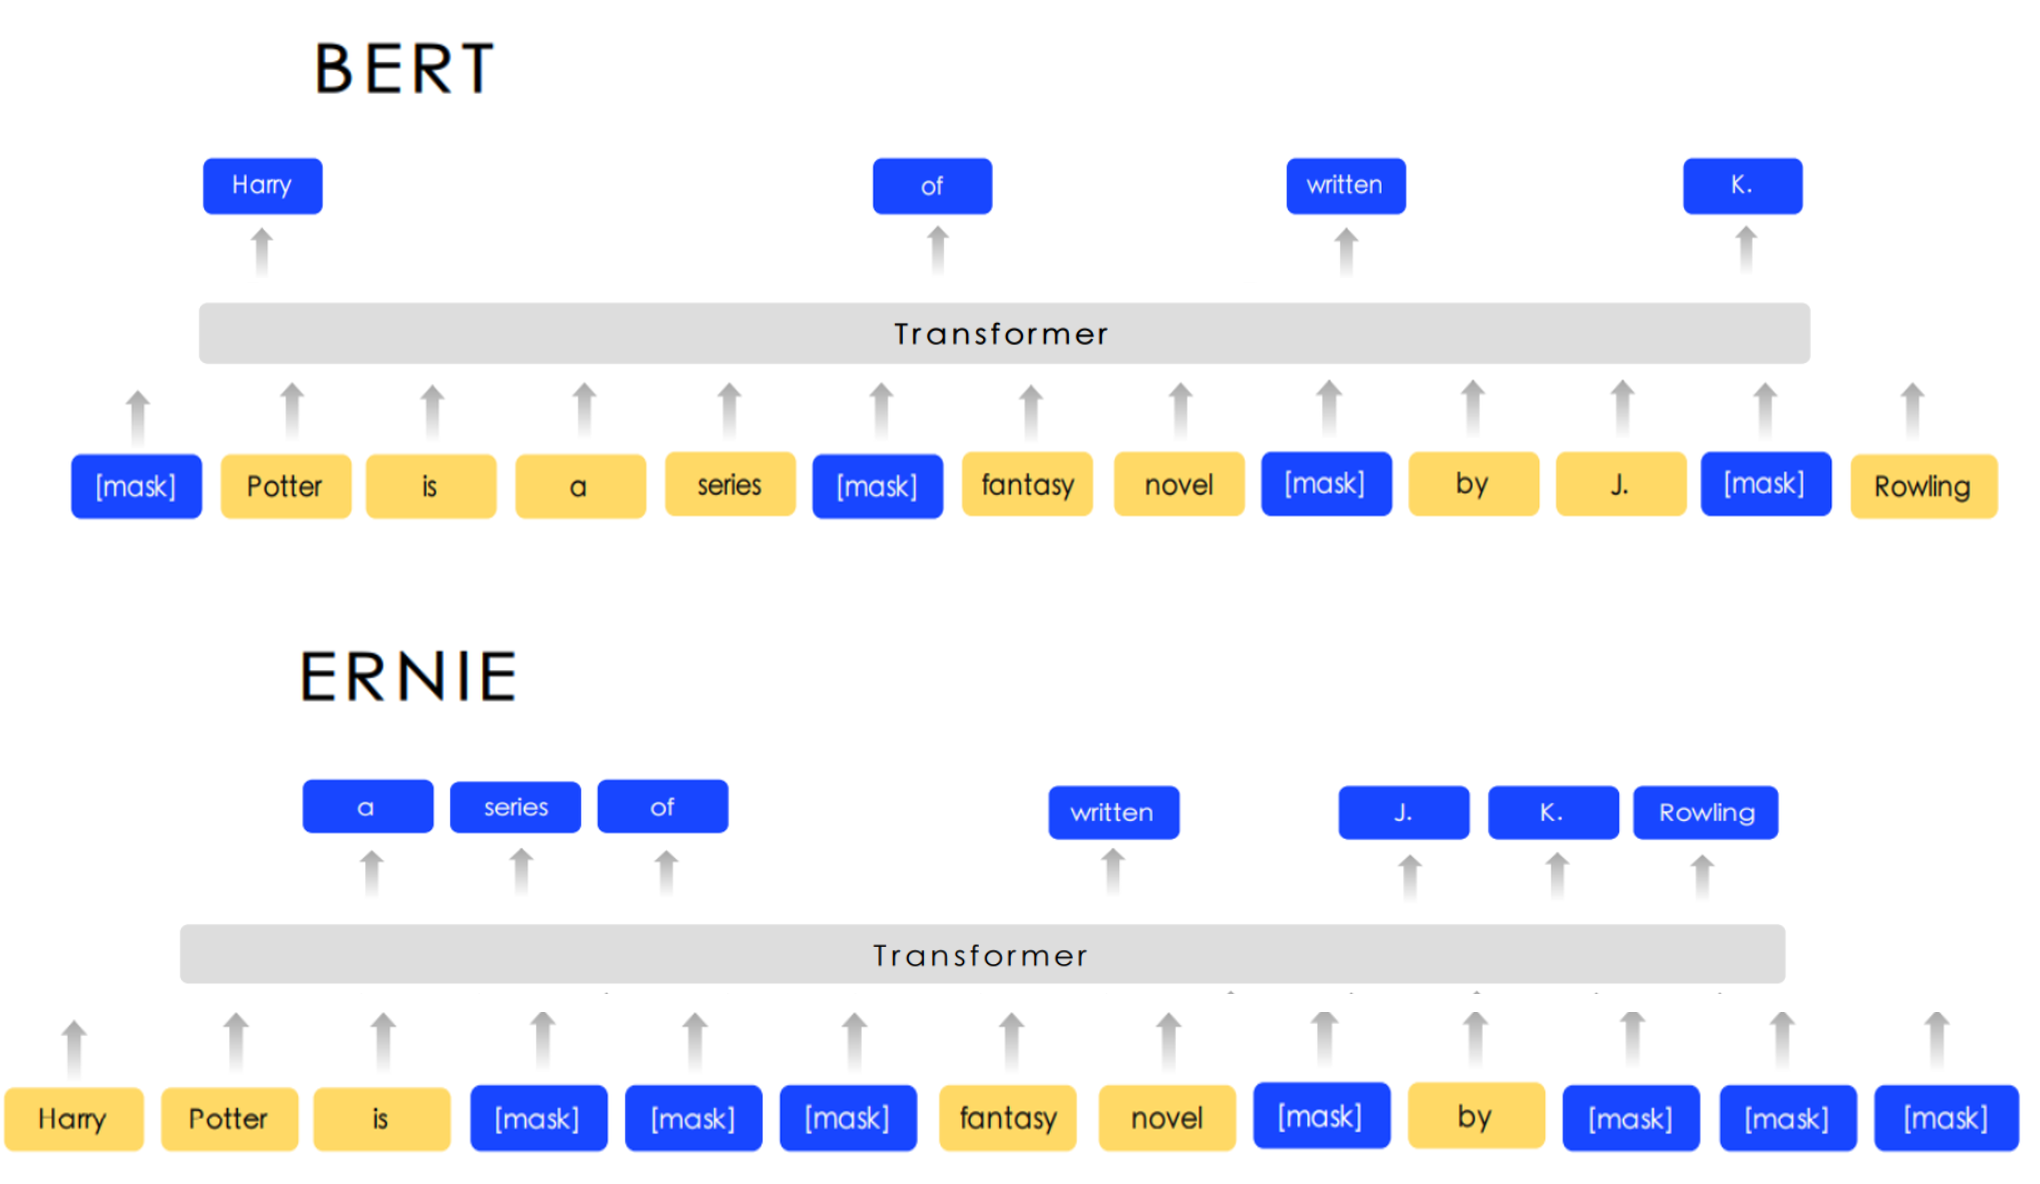
\includegraphics[width=0.9\textwidth]{imgs/ernie_vs_bert_masking.png}
%\vspace{-5pt}
%\captionof{figure}{  Conceptual difference between \nameref{sec:BERT}'s masking and ERNIE's masking. From \emph{ERNIE: Enhanced Representation Through Knowledge Integration}, by Sun et al., 2019a. \url{https://arxiv.org/pdf/1904.09223.pdf}. Copyright 2019a by Sun et al.}
%\vspace{-5pt}
%\label{fig:ernie_vs_bert_masking}
%\end{figure}


%ERNIE leverages a \nameref{sec:Transformer} encoder with \hyperref[sec:SelfAttention]{self-attention} alongside novel knowledge integration techniques like \nameref{sec:entitymasking} and \nameref{sec:phrasemasking} so that prior knowledge contained in conceptual units like phrases and entities can contribute to learning longer semantic dependencies for better model generalization and adaptability (Sun et al., 2019a). 





\begin{figure}[h]
\vspace{-5pt}
\centering
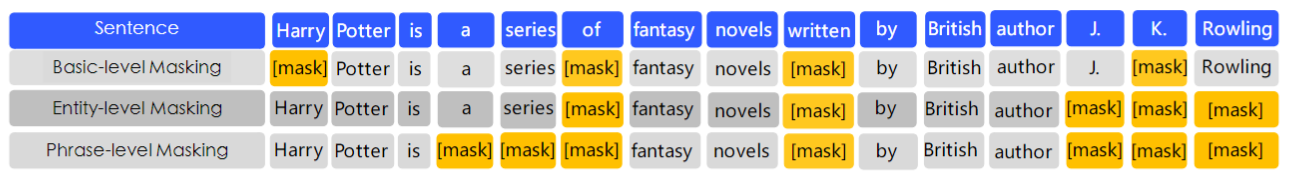
\includegraphics[width=0.99\textwidth]{imgs/ernie_maskingtypes.png}
\vspace{-5pt}
\captionof{figure}{ERNIE 1.0 uses basic masking to get word representations, followed by phrase-level and entity-level masking. From \emph{ERNIE: Enhanced Representation Through Knowledge Integration}, by Sun et al., 2019. \url{https://arxiv.org/pdf/1904.09223.pdf}. Copyright 2019 by Sun et al.}
\vspace{-5pt}
\label{fig:ernie_maskingTypes}
\end{figure}




\subsubsection{phrase-level masking}\label{sec:phrasemasking}

A phrase is a ``small group of words of characters together acting as a conceptual unit" (Sun et al., 2019a). ERNIE chunks sentences by phrase boundaries, then does phrase-masking by randomly selecting phrases, masking them, and training to predict subpieces of the phrase. This way, phrase information gets built into ERNIE's embeddings. 


\subsubsection{entity-level masking}\label{sec:entitymasking}

From Sun et al. (2019a), name entities contain ``persons, locations, organizations, products" that are denoted with a proper name, and can be abstract or have physical existence. Entities often contain important information within a sentence, so are regarded as conceptual units. ERNIE parses a sentence for its named entities, then masks and predicts all slots within the entities, as in \cref{fig:ernie_maskingTypes}.


\subsection{Experimental Results of ERNIE 1.0}\label{sec:ExperimentalResultsERNIE}


{
\begin{wrapfigure}{L}{0.7\textwidth}
\begin{center}
    \vspace{-30pt}
    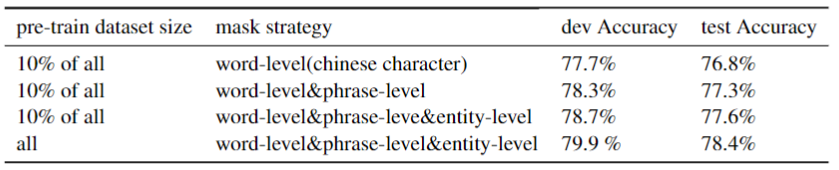
\includegraphics[width=\linewidth]{imgs/ernie_tableAblation.png}
\end{center}
\vspace{-20pt}
\captionof{table}{Ablation study for ERNIE's \nameref{sec:phrasemasking} and \nameref{sec:entitymasking}. From Table 2 in \emph{ERNIE: Enhanced Representation Through Knowledge Integration}, by Sun et al., 2019. \url{https://arxiv.org/pdf/1904.09223.pdf}. Copyright 2019 by Sun et al.}
%\vspace{-45pt}
%\vspace{10pt}
\label{tbl:ernie_ablationStudy}
\end{wrapfigure}

Sun et al. (2019a) show that ERNIE 1.0 outperforms \nameref{sec:BERT} by more than $1 \%$ absolute accuracy on five Chinese NLP tasks: \nameref{nlptask:naturallanguageinferenceNLI} (XNLI data), \nameref{nlptask:semantictextualsimilaritySTS} (LCQMC data), \nameref{nlptask:namedentityrecognitionNER} (MSRA-NER data), \nameref{nlptask:sentimentanalysisSA} (ChnSentiCorp data), \nameref{nlptask:questionansweringQA} (NLPCC-DBQA data).

Evidence of the superiority of ERNIE's knowledge integration strategy is visible in \cref{tbl:ernie_ablationStudy}, which shows that adding phrase masking to basic word-level masking improved ERNIE's performance almost a full percent, and adding entity masking to this combination resulted in still higher gains for larger data.
}



Additionally, the authors tested ERNIE's knowledge learning ability using fill-in-the-blanks on named entities in paragraphs. In case 1 from \cref{tbl:ernie_vs_bert_knowledgeLearningTask}, ERNIE predicts the correct father name entity based on prior knowledge in the article while \nameref{sec:BERT} simply memorizes one of the sons' name, completely ignoring any relationship between mother and son. In case 2, \nameref{sec:BERT} outputs some characters from contextual patterns it learned, but cannot even fill the slot with an entity, while ERNIE fills the slots with the \emph{correct} entity. In cases 3,4,6 \nameref{sec:BERT} once more fills the slots with characters related to the sentences but not with the semantic concept, while ERNIE again predicts the correct entities. However in case 4, even though ERNIE predicts the wrong city name, it still understands the semantic type is a city. Evidently, ERNIE's contextual knowledge understanding is far superior to \nameref{sec:BERT}'s predictions (Sun et al., 2019a). 



\begin{table}[htbp]
   % \scriptsize 
    \centering 
    \linespread{0.5}
    \setlength{\tabcolsep}{4pt} % Default value: 6pt
    \renewcommand{\arraystretch}{3} % Default value: 1
    
    \begin{tableFont}
    \begin{tabu} to \textwidth {| X[0.4] | X[6] | X | X | X |}
        
    
        \hline
      
        %\rowcolor{MyLavender} 
        \centering \textbf{Case}
        & \centering \textbf{Text} 
        & \centering \textbf{ERNIE}
        & \centering\textbf{BERT} 
        & \centering \textbf{Answer} \\ 
        
        \hline
        
        
        $1$
        &
        ``In September 2006, $\_\_\_$ married Cecilia Cheung. They had two sons, the older one is Zhenxuan Xie and the younger one is Zhennan Xie." \newline
        & 
        Tingfeng Xie
        & 
        Zhenxuan Xie
        & 
        {\color{Green} \textbf{Tingfeng Xie}} \\ 
        
        \hline 
        
        
        
        $4$
        &
        ``Australia is a highly developed capitalist country with $\_\_\_$ as its capital. As the most developed country in the Southern Hemisphere, the $12$th largest economy in the world and the fourth largest exporter of agricultural products in the world, it is also the world's largest exporter of various minerals."   \newline 
        & 
        Melbourne
        & 
        (Not a city name)
        & 
        {\color{Green} \textbf{Canberra}} \\ 
        
        \hline 
        
        $6$
        &
        ``Relativity is a theory about space-time and gravity, which was founded by $\_\_\_$."   
        & 
        Einstein
        & 
        (Not a word in Chinese)
        & 
        {\color{Green} \textbf{Einstein}} \\ 
        
        
        \hline 
    \end{tabu}
    
    \end{tableFont}
    
    \vspace{-5pt}
    
    \captionof{table}{Comparing ERNIE to BERT on Cloze Chinese Task. From Figure 4 in \emph{ERNIE: Enhanced Representation Through Knowledge Integration}, by Sun et al., 2019a. Copyright 2019 by Sun et al.}
    
    \label{tbl:ernie_vs_bert_knowledgeLearningTask}
\end{table}

